\documentclass[11pt]{article}
\usepackage{icmlko}
\begin{document}

\title{만화의 유보가 여섯 행인 것은 자료가 없어서가 아니었다}
\author{월드모델 실험실}
\date{노트 365 · 2026년 8월 1일}
\maketitle

\begin{abstract}
노트 364가 만화 문제를 회계로 정리했다 --- 만화는 남에게 $+0.0035$ 를
물리면서 유보 6행이라 한 번도 채점이 안 되고, 그래서 아무 값도 안 낸다.
\textbf{닫는 길은 만화를 채점되게 만드는 것이고, 노트 356은 그것을
``2026년 만화 레코드가 아예 없다''로 적어 뒀다.} 왜 없는지 봤다 ---
\texttt{ingest/manga\_domain} 의 질의가 \texttt{sort: POPULARITY\_DESC} 로
상위 2,000건을 훑는다. \textbf{최근작은 아직 인기가 없어서 구조적으로
빠진다.} 자국이 깨끗하다: 축 파일의 2025년 이후 6건이 \emph{새로 긁은
258건 중 인기 상위 여섯}과 정확히 일치한다. \texttt{startDate\_greater} 로
따로 긁으니 JP 2025년 이후 \textbf{258건}이 나왔고, 시계 검사도 통과한다
(달력 기준선 $0.20$, 학습 $-0.159$ 대 유보 $-0.202$).
\textbf{그런데 넣으니 축이 하나 조용히 사라졌다.} 만화 \texttt{media\_push}
가 학습 덮음 100\%에서 \textbf{0\%}가 된다 --- 그 축은
\texttt{media\_push\_fill.json} 이 채우는데, 파일에 \texttt{ids} 가 있는데도
읽는 쪽이 \emph{자리}로 붙이고 길이가 어긋나면 \texttt{continue} 로 조용히
버린다(1,789 대 2,041). \textbf{아홉 번째 갈라진 목록이고, 이번엔 쓰는 쪽이
키를 적어 뒀는데 읽는 쪽이 안 쓴 경우다.} 되돌렸다.
\end{abstract}

\section{왜 2026년 만화가 없었나}

\begin{center}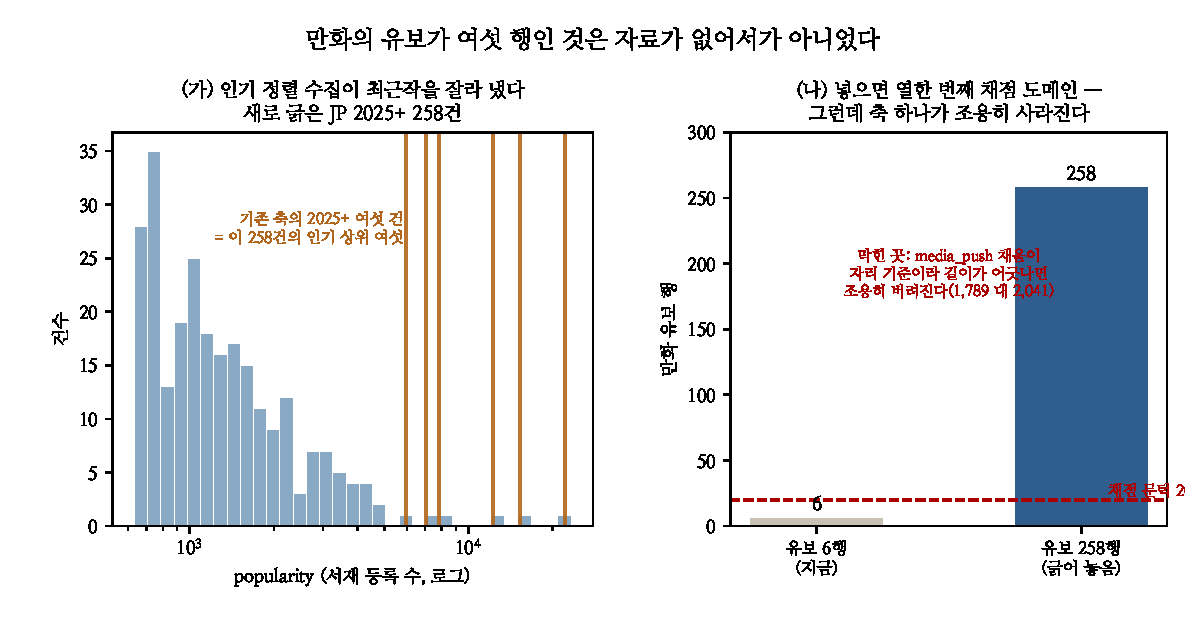
\includegraphics[width=\linewidth]{figs/recency.pdf}\end{center}

\texttt{manga\_domain.Q} 는 이렇다.
\begin{center}
\texttt{media(type: MANGA, sort: POPULARITY\_DESC)}
\end{center}
인기 순으로 2,000건을 받는다. \textbf{신작은 아직 인기가 없다.} 그래서
2023년 53건 · 2024년 21건 · 2025년 6건 · 2026년 0건으로 최근으로 갈수록
말라 간다.

\textbf{증거가 깨끗하다.} \texttt{startDate\_greater: 20250101} 로 따로
긁어 JP 2025년 이후 258건을 받았는데, \emph{기존 축 파일에 있던 2025년
이후 6건이 그 258건의 인기 상위 여섯}이다(popularity 5,963\textasciitilde{}22,154
대 258건의 99분위 9,819). 만화의 유보는 ``최근 만화 여섯 건''이 아니라
\textbf{``최근 만화 중 제일 유명한 여섯 건''}이었다.

\textbf{같은 집안이 셋째다.} 노트 209 · 269의 도서(베스트셀러 스크랩이라
``2020년 이전''이 ``지금도 잘 팔리는 옛 책''), 노트 357의 팝업(계수 방법
필터가 209행을 통째로 뺌), 그리고 여기. \textbf{수집 순서가 과제를 정한다.}

\section{시계 검사는 통과한다}

라벨이 누적 서재 등록 수라 최근작이 불리하다. 노트 209 · 269 · 270의
검사를 걸었다.

\begin{center}
\begin{tabular}{lr}
\hline
학습(1,783행) 시작일 $\leftrightarrow$ 라벨 & $-0.159$ \\
유보(258행) 시작일 $\leftrightarrow$ 라벨   & $-0.202$ \\
달력 기준선($-$시작일 하나) & $\mathbf{0.202}$ \\
\hline
\end{tabular}
\end{center}

학습과 유보의 시계가 비슷하고 달력 기준선이 0.20이다 --- 노트 269의
도서(달력 $0.5615$ 가 모형 $0.3480$ 을 이겼다)와 다르다. 반년 사분위별
라벨 중앙도 $1301 \to 1277 \to 1102 \to 1021$ 로 18개월에 1.27배다.

\section{넣어 봤더니 축이 하나 사라졌다}

넣으면 만화가 유보 258행으로 열한 번째 채점 도메인이 된다. 돌렸다 ---
만화 $\rho = 0.2545$, 95\% $[0.140,\,0.366]$(폭 0.226 으로 판에서 넷째로
좁다), 판 $0.4862 \to 0.4624$(분모 $2{,}723 \to 2{,}981$), 못 가리는 쌍
$30/45 \to 32/55$(비율 67\% $\to$ 58\%).

\textbf{그런데 다른 도메인이 움직였다} --- 게임 $0.5903 \to 0.5697$ ·
도서 $0.4349 \to 0.3921$. 새 레코드는 전부 2025년 이후라 학습에 안
들어가므로 \emph{모형이 같아야} 한다. 사전 등록에 그렇게 적었다. 틀렸다.

찾아보니 만화 \texttt{media\_push} 의 학습 덮음이 \textbf{100\% $\to$ 0\%}
가 됐다. 그 축은 \texttt{ingest/manga\_axes} 가 아니라
\texttt{state/tri\_domain.\_apply\_adopted} 가 \texttt{media\_push\_fill.json}
으로 채운다(노트 108). 그 코드는 이렇다.

\begin{center}
\texttt{if len(v) != len(y): continue}
\end{center}

\textbf{파일에는 \texttt{ids} 가 들어 있다}(만화 1,789개 · 세계애니
2,948개). 그런데 읽는 쪽은 그 키를 안 쓰고 \emph{자리}로 붙인다. 행이
2,041로 늘자 길이가 어긋났고, 예외도 경고도 없이 축 하나가 통째로
빠졌다. \textbf{아홉 번째 갈라진 목록이다} --- 그리고 앞의 여덟과 다르다.
지금까지는 한쪽이 키를 안 적어서 갈라졌는데, \textbf{여기는 쓰는 쪽이
키를 적어 뒀고 읽는 쪽이 안 썼다.}

\textbf{되돌렸다.} 판 0.4862 · 분모 2,723 · 만화 \texttt{media\_push}
덮음 1.000 으로 복원을 확인했다.

\section{왜 지금 안 고치나}

\texttt{\_apply\_adopted} 를 id 기준으로 고치는 것은 세 줄이다. 그런데
그러면 \textbf{새 258행은 \texttt{media\_push} 가 결측}이 되고, 그 결측
무늬가 곧 ``2025년 이후인가''가 된다 --- 노트 354가 시장팝업에서 잡은
\emph{배치 표시자}와 정확히 같은 덫이고 노트 214의 한철 가드가 잡을
자리다. 그러니 id 로 고치는 것만으로는 안 되고 \textbf{새 258건의
\texttt{media\_push} 를 실제로 채워야} 한다.

채우는 개념은 노트 108의 주석에 남아 있다 --- ``공식 외부 채널 수와
예고편 유무''. 그런데 \textbf{그것을 만든 스크립트가 저장소에 없다.}
남은 것은 출력 파일뿐이고, 값이 21개 구간으로 뭉쳐 있어(0.0419 · 0.1515 ·
0.3077 $\cdots$) 눈금을 역산해 맞추는 것은 추측이 된다. \textbf{추측한
눈금으로 옛 값과 새 값을 섞으면 노트 357이 팝업에서 본 기준 섞임을 내가
만드는 것이다.}

\textbf{그래서 이번 사이클에서는 안 넣는다.} 할 일이 분명해졌다는 것이
이 노트의 결과다.

\section{규약에 더하는 줄}

\begin{itemize}
\item \textbf{키가 있는데 자리로 붙이지 마라.} 그리고 길이가 어긋날 때
\texttt{continue} 로 넘어가면 축이 조용히 사라진다 --- 최소한 경고를
남긴다.
\item \textbf{수집 정렬이 과제를 정한다.} 인기순 · 베스트셀러 · 계수 방법
--- 세 도메인에서 같은 일이 났다. \emph{무엇으로 정렬해 모았나}를 도메인
문서에 적는다.
\item \textbf{``자료가 없다''를 믿기 전에 어떻게 모았는지 본다.} 만화
2026년 0건은 없어서가 아니라 인기순이어서였다.
\end{itemize}

\section{남은 것}

\begin{center}
\begin{tabular}{ll}
\hline
갈래 & 지금 아는 것 \\
\hline
\textbf{만화 258행 넣기} & \texttt{media\_push} 를 258건에 채우면 끝난다. \\
 & AniList \texttt{externalLinks}/\texttt{trailer} 재수집 \\
 & $+$ 눈금 재정의(옛 값도 같이 다시 만든다) \\
\texttt{\_apply\_adopted} 를 id 로 & 세 줄. 다만 위와 같이 해야 안전하다 \\
팝업 실측 41행 & 노트 360. 결정 넷을 다 팝업이 내렸다 \\
세계애니 fill 도 자리 기준 & 2,948행. 같은 덫이 하나 더 걸려 있다 \\
\hline
\end{tabular}
\end{center}

마지막 줄이 새로 보인다 --- 세계애니도 같은 파일 · 같은 코드 경로다.
그 도메인의 행 수가 바뀌는 날 같은 일이 난다.

\end{document}
